\documentclass[a4paper, 11pt]{article}
\usepackage[margin=3cm]{geometry}
\usepackage[]{fontenc}
\usepackage[utf8]{inputenc}
\usepackage[italian]{babel}
\usepackage{geometry}
\geometry{a4paper, top=2cm, bottom=3cm, left=1.5cm, right=1.5cm, heightrounded, bindingoffset=5mm}
\usepackage{amsmath}
\usepackage{amssymb}
\usepackage{gensymb}
\usepackage{graphicx}
\usepackage{psfrag,amsmath,amsfonts,verbatim}
\usepackage{xcolor}
\usepackage{color,soul}
\usepackage{fancyhdr}
\usepackage{indentfirst}
\usepackage{graphicx}
\usepackage{newlfont}
\usepackage{amssymb}
\usepackage{amsmath}
\usepackage{latexsym}
\usepackage{amsthm}
%\usepackage{subfigure}
\usepackage{subcaption}
\usepackage{psfrag}
\usepackage{footnote}
\usepackage{graphics}
\usepackage{color}
\usepackage{hyperref}
\usepackage{tikz}


\usetikzlibrary{snakes}
\usetikzlibrary{positioning}
\usetikzlibrary{shapes,arrows}

	
	\tikzstyle{block} = [draw, fill=white, rectangle, 
	minimum height=3em, minimum width=6em]
	\tikzstyle{sum} = [draw, fill=white, circle, node distance=1cm]
	\tikzstyle{input} = [coordinate]
	\tikzstyle{output} = [coordinate]
	\tikzstyle{pinstyle} = [pin edge={to-,thin,black}]

\newcommand{\courseacronym}{CAT}
\newcommand{\coursename}{Controlli Automatici - T}
\newcommand{\tipology}{b }
\newcommand{\trace}{1}
\newcommand{\projectname}{Controllo di meccanismo non-lineare attuato}
\newcommand{\group}{K}

%opening
\title{ \vspace{-1in}
		\huge \strut \coursename \strut 
		\\
		\Large  \strut Progetto Tipologia \tipology - Traccia \trace 
		\\
		\Large  \strut \projectname\strut
		\\
		\Large  \strut Gruppo \group\strut
		\vspace{-0.4cm}
}
\author{Lorenzo Venturoli, Leonardo Benini, Gianluca Sabatini}
\date{}

\begin{document}

\maketitle
\vspace{-0.5cm}

Il progetto riguarda il controllo di un sistema a meccanismo motorizzato di Figura \ref{fig:system_image}, la cui dinamica viene descritta dalle seguenti equazioni differenziali  
%
\begin{subequations}\label{eq:system}
\begin{align}
	J(\theta) = \dot{\omega} = C_m - \beta\omega - k\theta 
\end{align}
\begin{align}
	J(\theta) = J_0 + \sum_{n = 0}^{4}J_i\cos (i\theta +\psi_i)
\end{align}
\end{subequations}
%
dove $\omega$(t) rappresenta la velocità angolare e in cui:
\begin{itemize}
	\item il momento d'interzia ridotto al movente $J(\theta)$ è una funzione periodica di periodo 2$\pi$;
	\item $C_m$ è la coppia generata dal motore elettrico;
	\item $\beta$ è l'attrito viscoso;
	\item k è il coefficiente di elasticità del disco;
  \end{itemize}
%
\begin{figure}[h!]
	\centering
	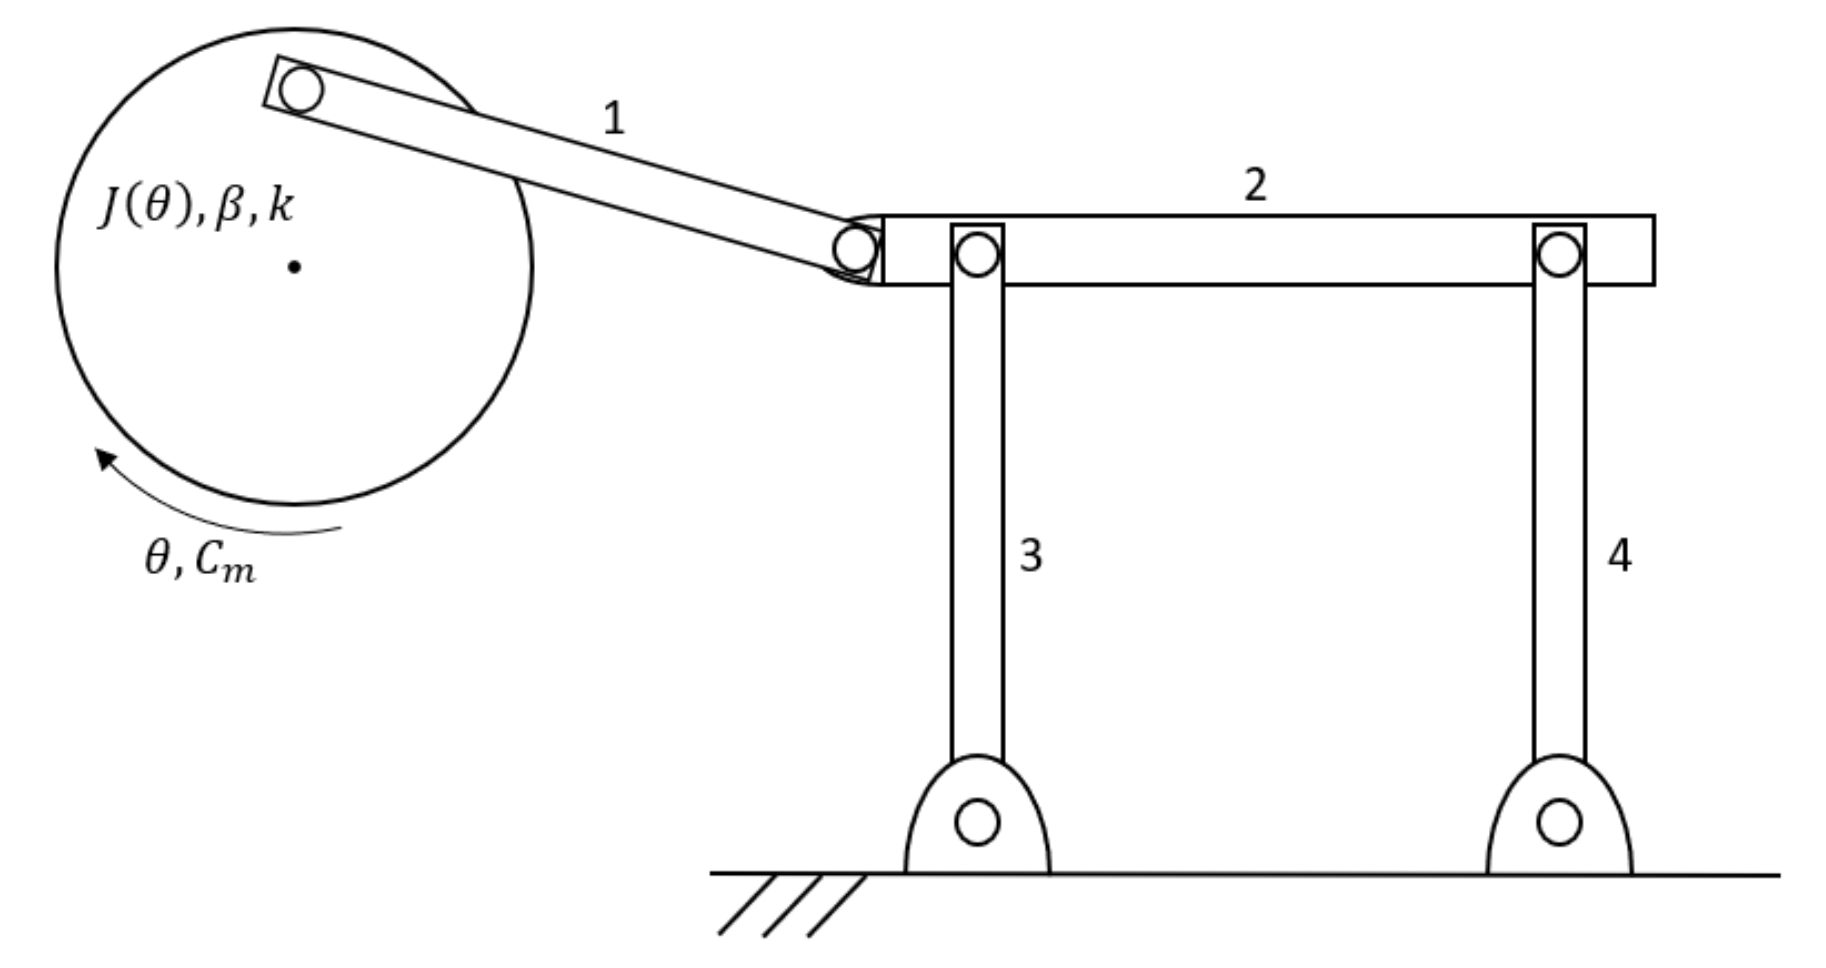
\includegraphics[width=0.75\linewidth]{./images/system_image.png}
	\caption{Schema illustrativo del sistema meccanismo motorizzato.}
	\label{fig:system_image}
\end{figure}
\section{Espressione del sistema in forma di stato e calcolo del sistema linearizzato intorno ad una coppia di equilibrio}

Innanzitutto, esprimiamo il sistema~\eqref{eq:system} nella seguente forma di stato
%
\begin{subequations}
\begin{align}\label{eq:state_form}
	\dot{x} &= f(x,u)
	\\
	y &= h(x,u).
\end{align}
\end{subequations}
%
Pertanto, andiamo individuare lo stato $x$, l'ingresso $u$ e l'uscita $y$ del sistema come segue 
%
\begin{align*}
	x := \left [ \theta, \omega \right ]^T, \quad u := C_m , \quad y := \theta.
\end{align*}
%
Coerentemente con questa scelta, ricaviamo dal sistema~\eqref{eq:system} la seguente espressione per le funzioni $f$ ed $h$
%
\begin{align}
	f(x,u) &:= 
	\begin{bmatrix}
		f_1(x,u)
		\\[0.5em] 
		f_2(x,u)
	\end{bmatrix} :=
	\begin{bmatrix}
		x_2
		\\[0.5em] 
		\dfrac{u - \beta x_2 - kx_1}{J(x_1)}
	\end{bmatrix}
	\\[0.5em] 
	h(x,u) &:= x_1
\end{align}
%
Una volta calcolate $f$ ed $h$ esprimiamo~\eqref{eq:system} nella seguente forma di stato
%
\begin{subequations}\label{eq:our_system_state_form}
\begin{align}
	\begin{bmatrix}
		\dot{x}_1
		\\
		\dot{x}_2
	\end{bmatrix} &= 
	\begin{bmatrix}
		f_1(x,u)
		\\[0.5em] 
		f_2(x,u)
	\end{bmatrix}\label{eq:state_form_1}
	\\[0.5em]
	y &= h(x, u)
\end{align}
\end{subequations}
%
Per trovare la coppia di equilibrio $(x_e, u_e)$ di~\eqref{eq:our_system_state_form}, andiamo a risolvere il seguente sistema di equazioni a partire dal valore fornito di $\theta_e=\frac{\pi}{3}$
%
\begin{align}
	\left\{\begin{matrix}
		f(x_e, u_e)=0  
		\\[0.5em]
		x_{e1} = \frac{\pi}{3}
	\end{matrix}\right.
\end{align}
%
dal quale otteniamo
%
\begin{align}
	x_e := \left[\frac{\pi}{3}, 0\right]^T,  \quad u_e = k\frac{\pi}{3}\label{eq:equilibirum_pair}
\end{align}
%
Definiamo le variabili alle variazioni $\delta x$, $\delta u$ e $\delta y$ come 
%
\begin{align*}
	\delta x &= x-x_e, 
	\quad
	\delta u = u-u_e, 
	\quad
	\delta y = y-y_e.
\end{align*}
%
L'evoluzione del sistema espressa nelle variabili alle variazioni pu\`o essere approssimativamente descritta mediante il seguente sistema lineare
%
\begin{subequations}\label{eq:linearized_system}
\begin{align}
	\delta \dot{x} &= A\delta x + B\delta u
	\\
	\delta y &= C\delta x + D\delta u,
\end{align}
\end{subequations}
%
dove le matrici $A$, $B$, $C$ e $D$ vengono calcolate come
%
\begin{subequations}\label{eq:matrices}
\begin{align}
	A &= \frac{\partial f(x, u)}{\partial x} \Bigg|_{\begin{smallmatrix}
		x = x_e
		\\
		u = u_e \end{smallmatrix}}
	\\
	B &= \frac{\partial f(x, u)}{\partial u} \Bigg|_{\begin{smallmatrix}
		x = x_e
		\\
		u = u_e \end{smallmatrix}}
	\\
	C &= \frac{\partial h(x, u)}{\partial x} \Bigg|_{\begin{smallmatrix}
		x = x_e
		\\
		u = u_e \end{smallmatrix}}
	\\
	D &= \frac{\partial h(x, u)}{\partial u} \Bigg|_{\begin{smallmatrix}
		x = x_e
		\\
		u = u_e \end{smallmatrix}}
\end{align}
\end{subequations}
%
\section{Calcolo Funzione di Trasferimento}

In questa sezione, andiamo a calcolare la funzione di trasferimento $G(s)$ dall'ingresso $\delta u$ all'uscita $\delta y$ mediante la seguente formula 
%
%
\begin{align}\label{eq:transfer_function}
G(s) = C(sI-A)^{-1}B + D = \frac{0.02}{1+0.09919\frac{s}{4.96}+\frac{s^2}{4.96^2}}
\end{align}
%
Dunque il sistema linearizzato~\eqref{eq:linearized_system} è caratterizzato dalla funzione di trasferimento~\eqref{eq:transfer_function} con 2 poli complessi coniugati $p_1$ e $p_2$:
\begin{align}
	p_1 = -0.2460 + 4.9536i, \quad p_2 = -0.2460 - 4.9536i
\end{align}
In Figura \ref{fig:G_bode} mostriamo il corrispondente diagramma di Bode. 

\begin{figure}[h!]
	\centering
	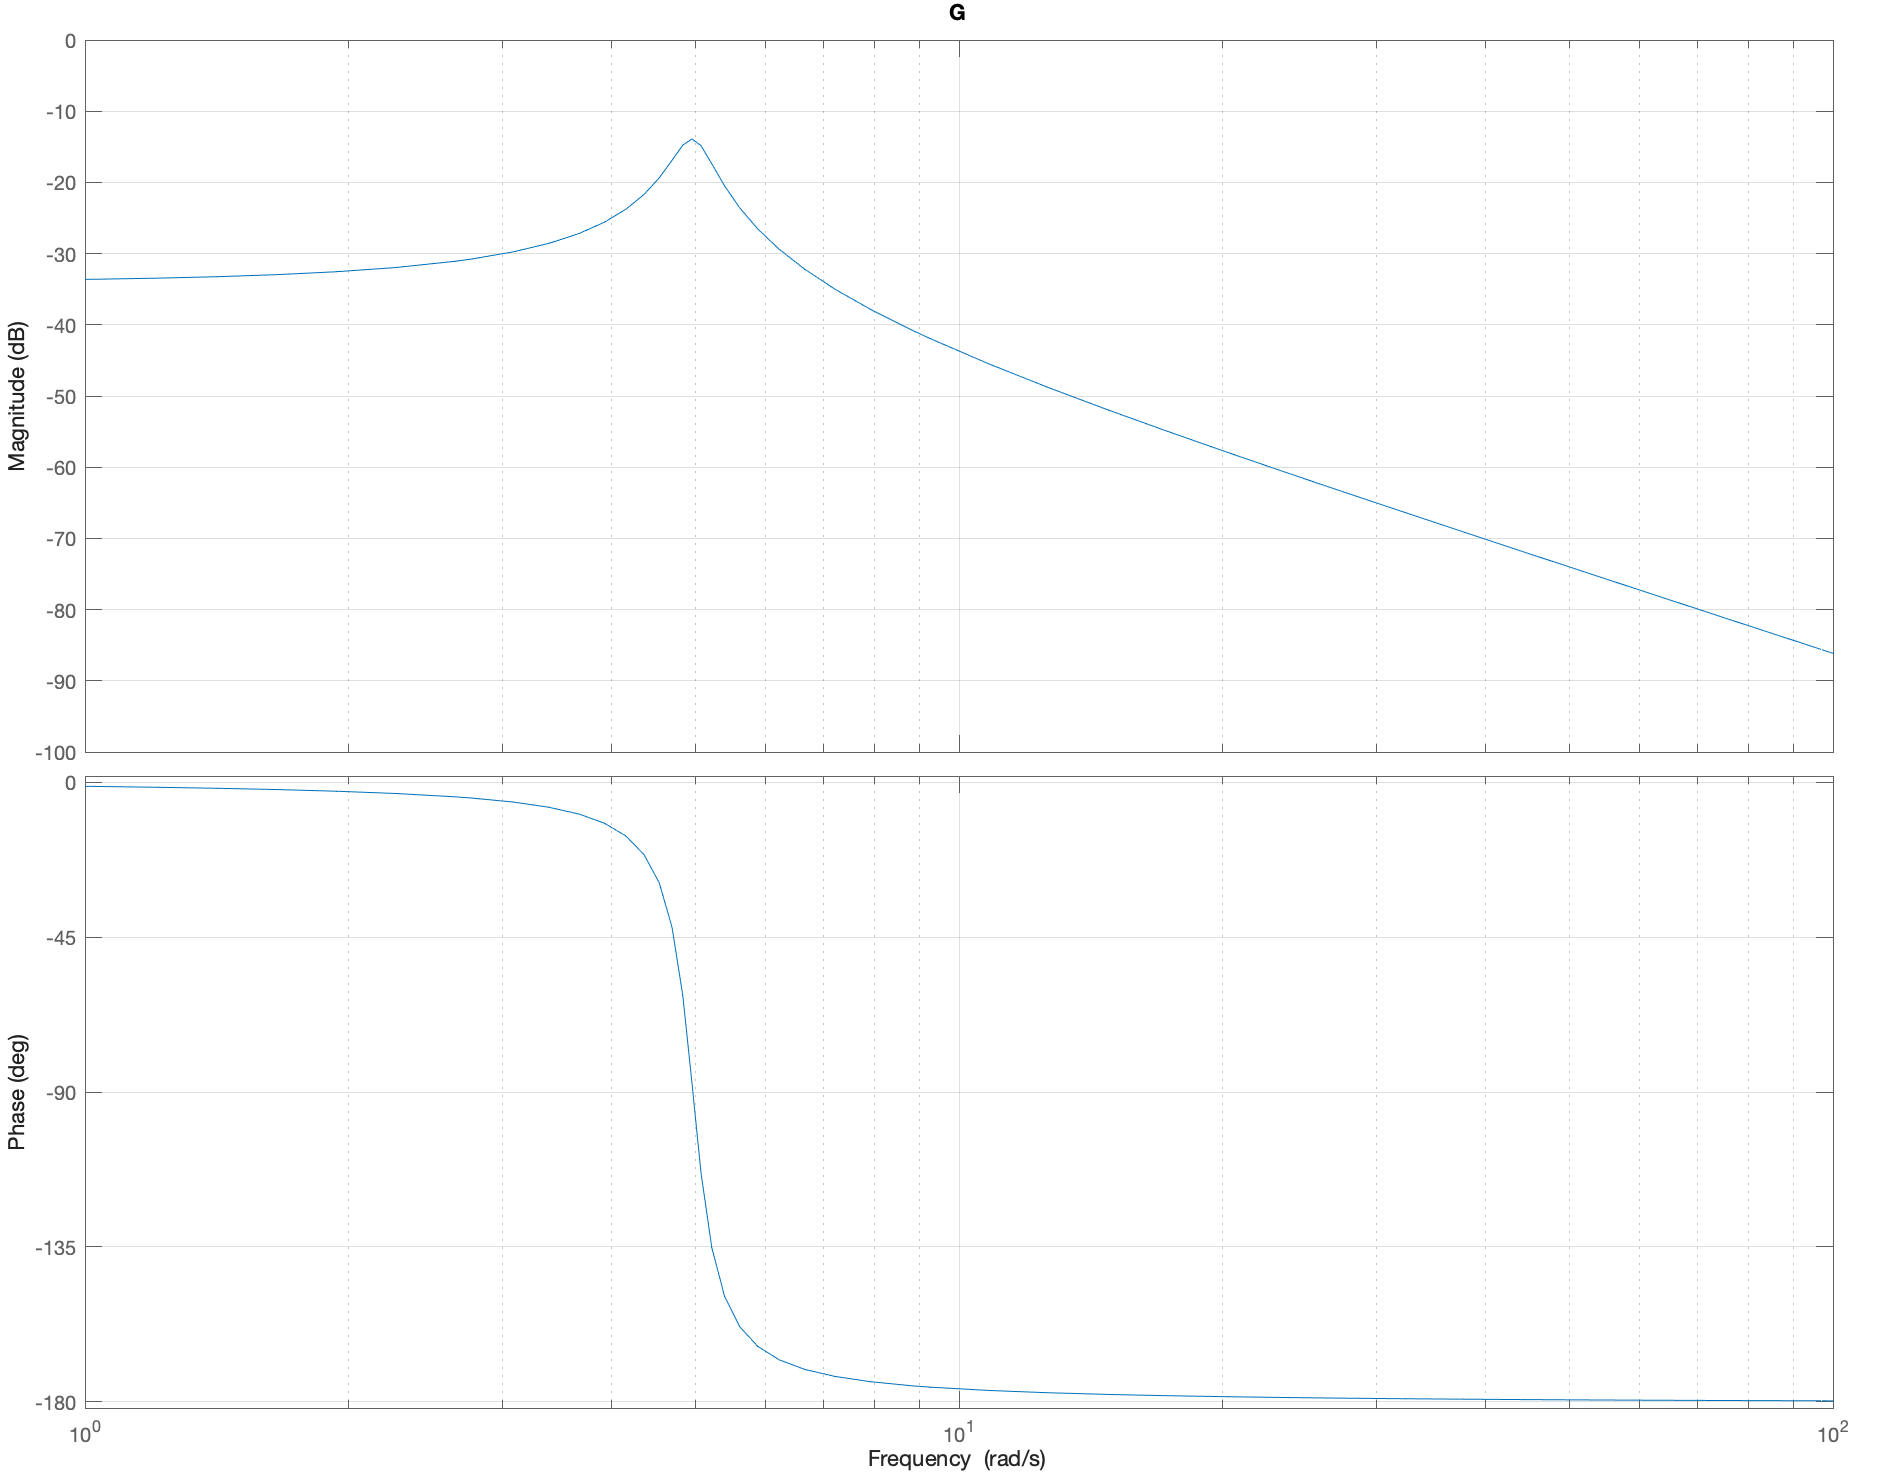
\includegraphics[width=0.75\linewidth]{./images/bode_G.png}
	\caption{Diagrammi di Bode della funzione di trasferimento G.}
	\label{fig:G_bode}
\end{figure}

\section{Mappatura specifiche del regolatore}
\label{sec:specifications}

Le specifiche da soddisfare sono
\begin{itemize}
	\item[1)] Errore a regime $|e_{\infty}| \leq e^{\star}$ in risposta a un gradino $\omega (t) = 1(t)$ e $d(t)=1(t)$
	\item[2)] Per garantire una certa robustezza del sistema si deve avere un margine di fase $M_f \geq 30^{\degree}$.
	\item[3)] Il sistema può accettare una sovraelongazione percentuale al massimo del 10\% : S\% $\leq 10\%$. 
	\item[4)] Il tempo di assestamento alla $\epsilon_{\%}$ = 5\% deve essere inferiore al valore fissato: $T_{a, \epsilon} = 0.008s$ .
	\item[5)] Il disturbo sull'uscita d(t), con una banda limitata nel range di pulsazioni $[0, 0.5]$, deve essere abbattuto di almeno 30 dB.
	\item[6)] Il rumore sull'uscita n(t), con una banda limitata nel range di pulsazioni $[5 \cdot 10^4, 5 \cdot 10^6]$, deve essere abbattuto di almeno 65 dB. 
\end{itemize}
%
Andiamo ad effettuare la mappatura punto per punto le specifiche richieste, tenendo a mente la fisica realizzabilità del regolatore \dots  

Pertanto, in Figura \ref{fig:G_bode_specifiche}, mostriamo il diagramma di Bode della funzione di trasferimento $G(s)$ con le zone proibite emerse dalla mappatura delle specifiche.
\begin{figure}[h!]
	\centering
	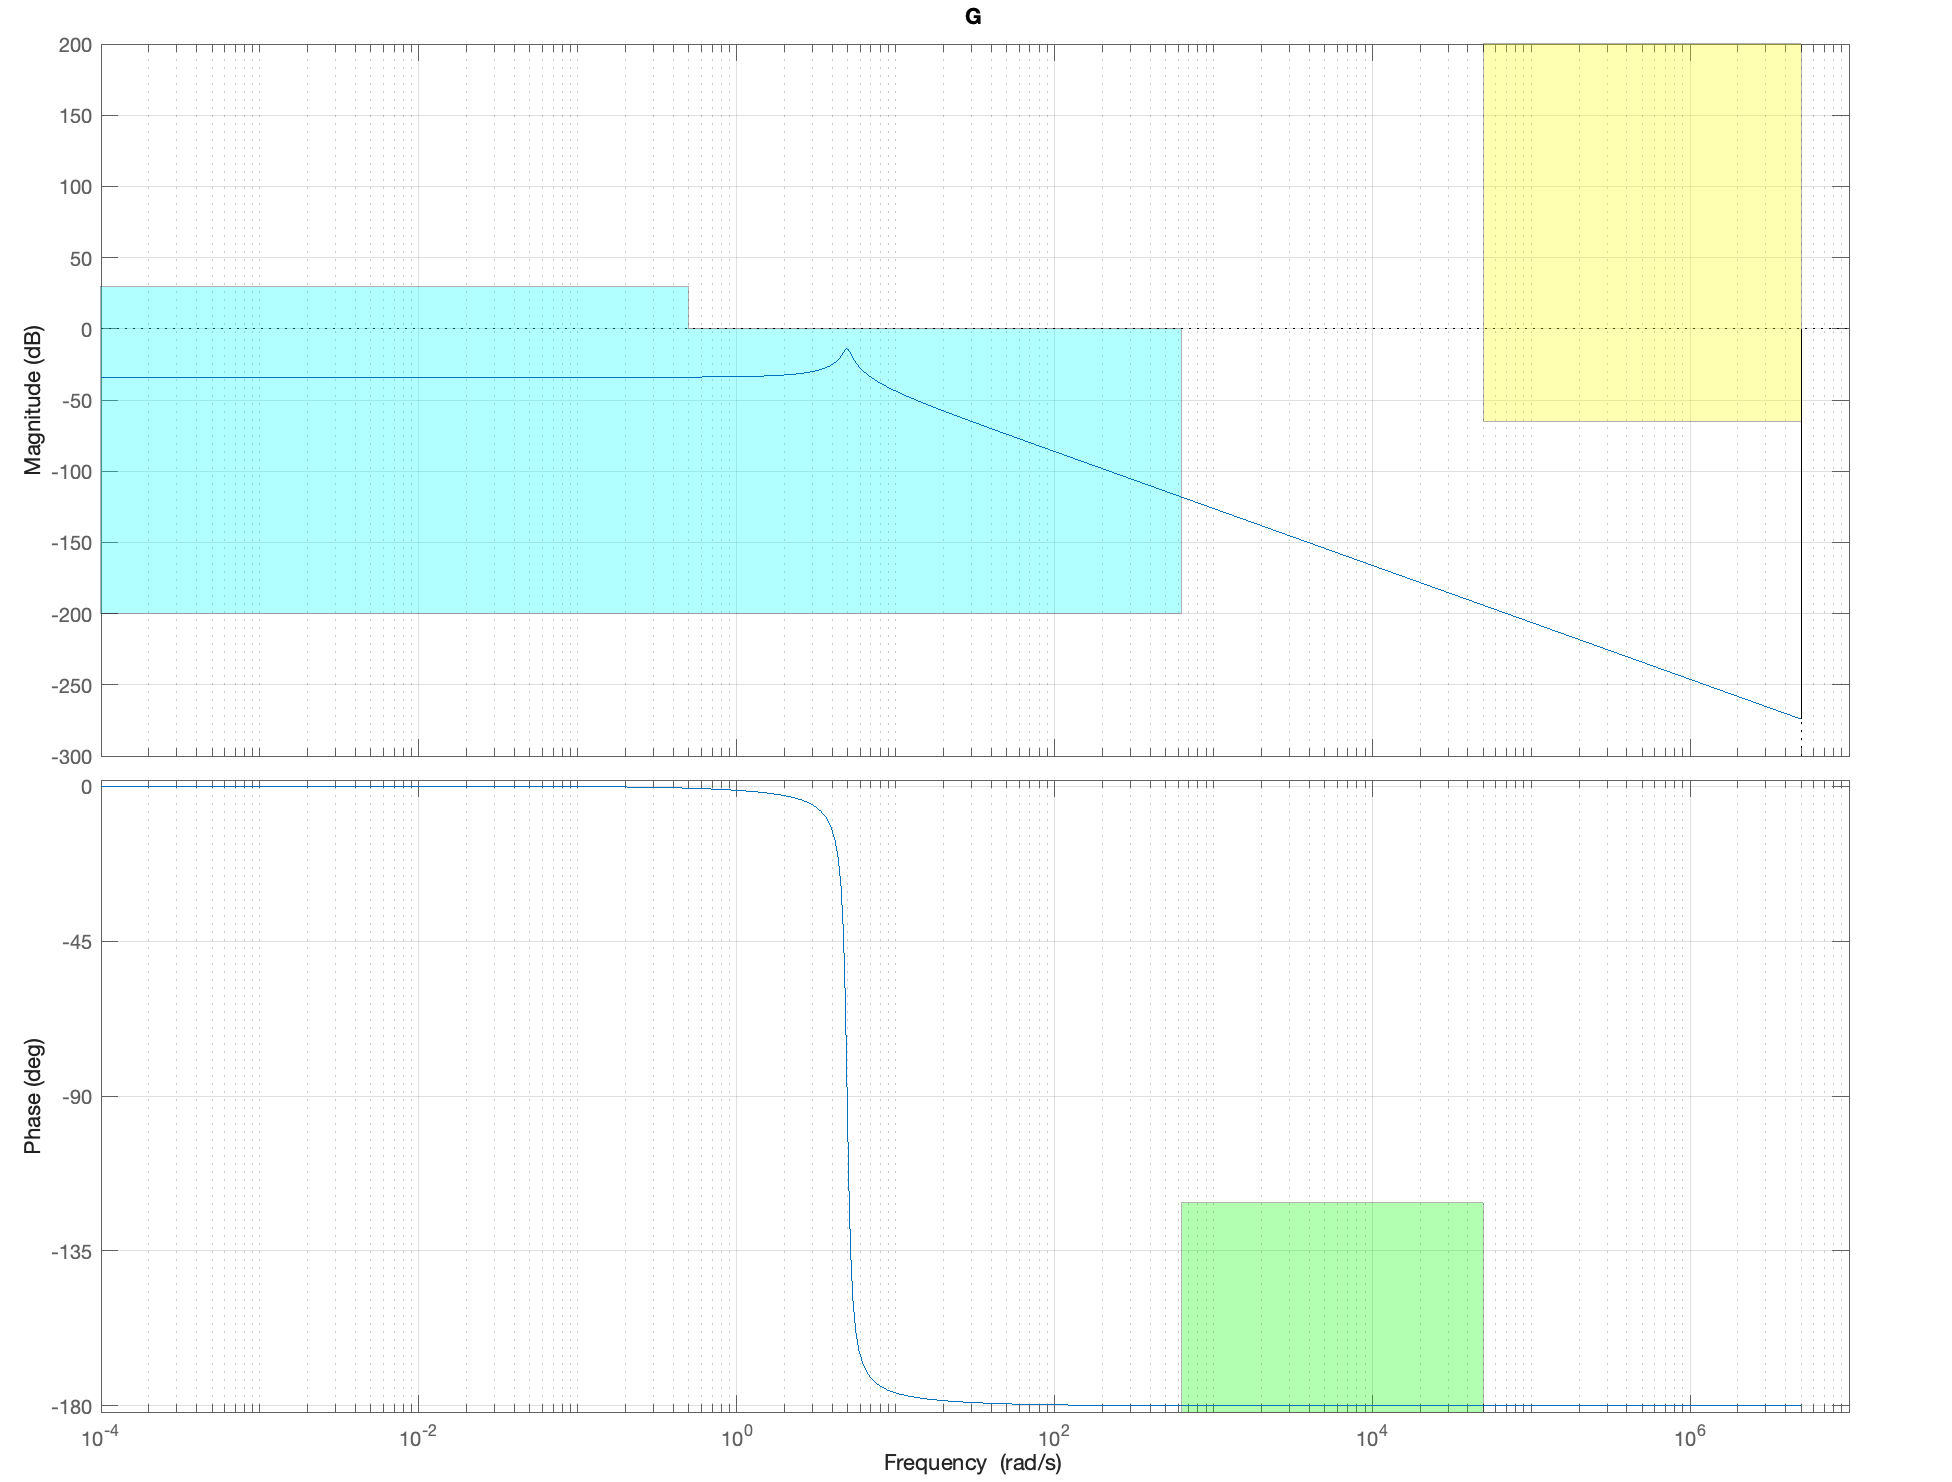
\includegraphics[width=0.75\linewidth]{./images/bode_G_mappatura.png}
	\caption{Mapputura delle specifiche.}
	\label{fig:G_bode_specifiche}
\end{figure}

\section{Sintesi del regolatore statico}
\label{sec:static_regulator}

In questa sezione progettiamo il regolatore statico $R_s(s)$ partendo dalle analisi fatte in sezione~\ref{sec:specifications}.

Nel nostro caso, essendo l'errore a regime $>$ 0 , possiamo progettare il regolatore statico come:
\begin{align}
	R(s) = \mu_s.
\end{align}

Consideriamo quindi che:
\begin{align}
	\mu_s \geq \mu^{\star} = \frac{D+W}{e^{\star}}.
\end{align}
Con D e W rispettive ampiezza dei gradini di disturbo sull'uscita e ingresso.\\
Per determinare $\mu_s$ bisogna anche considerare la specifica sull'attenuazione di d(t):
\begin{align}
	\mu_s \geq \mu_{sd} = 10^{\frac{A_d}{20}}.
\end{align}
Con $A_d$ pari a 30 dB. Otteniamo quindi $\mu_s$ come:
\begin{align}
	\mu_s \geq max\bigg(\frac{\mu^{\star}}{\left| L(0)\right|}, \frac{\mu_{sd}}{\left| G(j\omega_{d_{max}})\right|}\bigg).
\end{align}

Dunque, definiamo la funzione estesa $G_e(s) = R_s(s)G(s)$ e, in Figura \ref{fig:G_e}, mostriamo il suo diagramma di Bode per verificare se e quali zone proibite vengono attraversate.
Dalla figura emerge come il regolatore ora rispetti la specifica sull'attenuazione del disturbo in uscita.

\begin{figure}[h!]
	\centering
	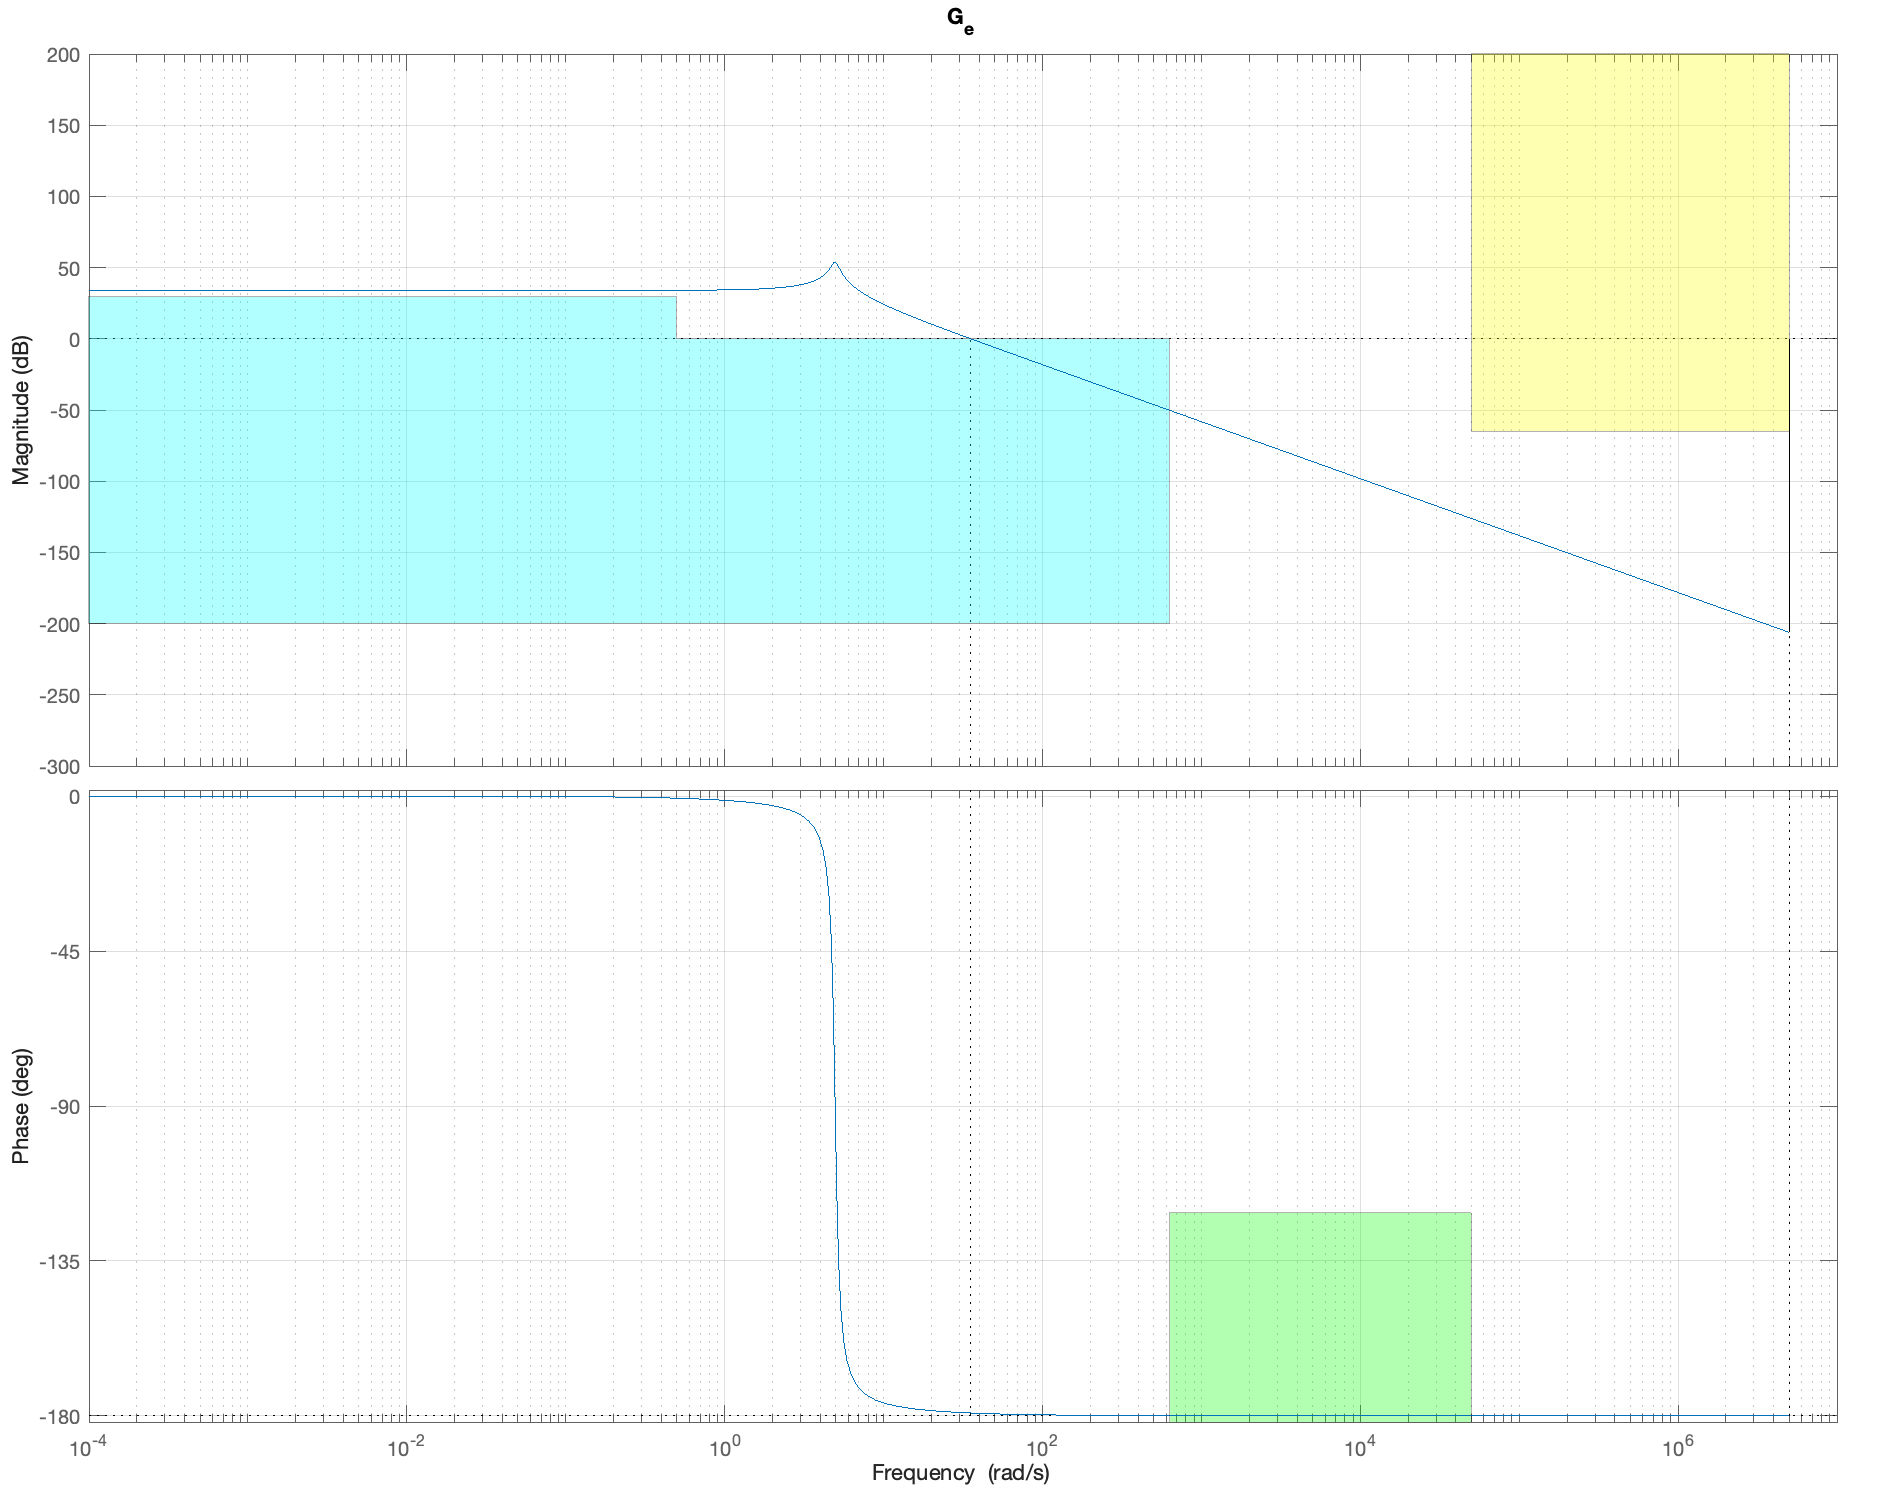
\includegraphics[width=0.75\linewidth]{./images/G_e.png}
	\caption{Mappatura specifiche su $G_e$.}
	\label{fig:G_e}
\end{figure}

\section{Sintesi del regolatore dinamico}
\label{sec:dynamic_regulator}

In questa sezione, progettiamo il regolatore dinamico $R_d(s)$. 
%
Dalle analisi fatte in Sezione~\ref{sec:static_regulator}, notiamo di essere nello Scenario di tipo B. Dunque, progettiamo $R_d(s)$ ricorrendo a una rete anticipatrice.\\
A questo scopo, calcoliamo il margine di fase per rispettare le specifiche:
\begin{align}
	\xi^{\star} = \sqrt[2]{\frac{\log{S}^2}{\pi^2 + \log{S}^2}}.
	\\[0.5em]
	Mf = max (\xi^{\star}, 30).
\end{align}
Dove S=0.1. Otteniamo quindi:
\begin{align}
	\omega_{c_{min}}=\frac{300}{T_{a, 5}*Mf}.
\end{align}
La rete anticipatrice si presenta nella forma:
\begin{align}
	R_d(s) = \frac{1+\tau s}{1+\alpha \tau s}.
\end{align}
Nel nostro caso, sfruttando le formule di inversione:
\begin{align}
	\tau = \frac{M^{\star}-\cos{\varphi^{\star}}}{\omega_c^{\star}\sin{\varphi^{\star}}}, \quad
	\alpha = \frac{\cos{\varphi^{\star}-\frac{1}{M^{\star}}}}{\omega_c^{\star}\sin{\varphi^{\star}}}\frac{1}{\tau}.
	\\[1em]
	M^{\star} = 10^{-\frac{\left|G_e(j\omega_c^{\star})\right|_{dB}}{20}}, \quad
	\varphi^{\star} = M_f^{\star} -\pi - \angle{G_e(j\omega_c^{\star})},
\end{align}
con $\omega_c^{\star}$ pari a 750 $\frac{rad}{s}$ e $M_f^{\star}$ pari a $M_f + 5$, da noi fissati rispettando le specifiche.\\

In Figura \ref{fig:funzione_anello}, mostriamo il diagramma di Bode della funzione d'anello $L(s) = R_d(s) G_e(s)$

\begin{figure}[h!]
	\centering
	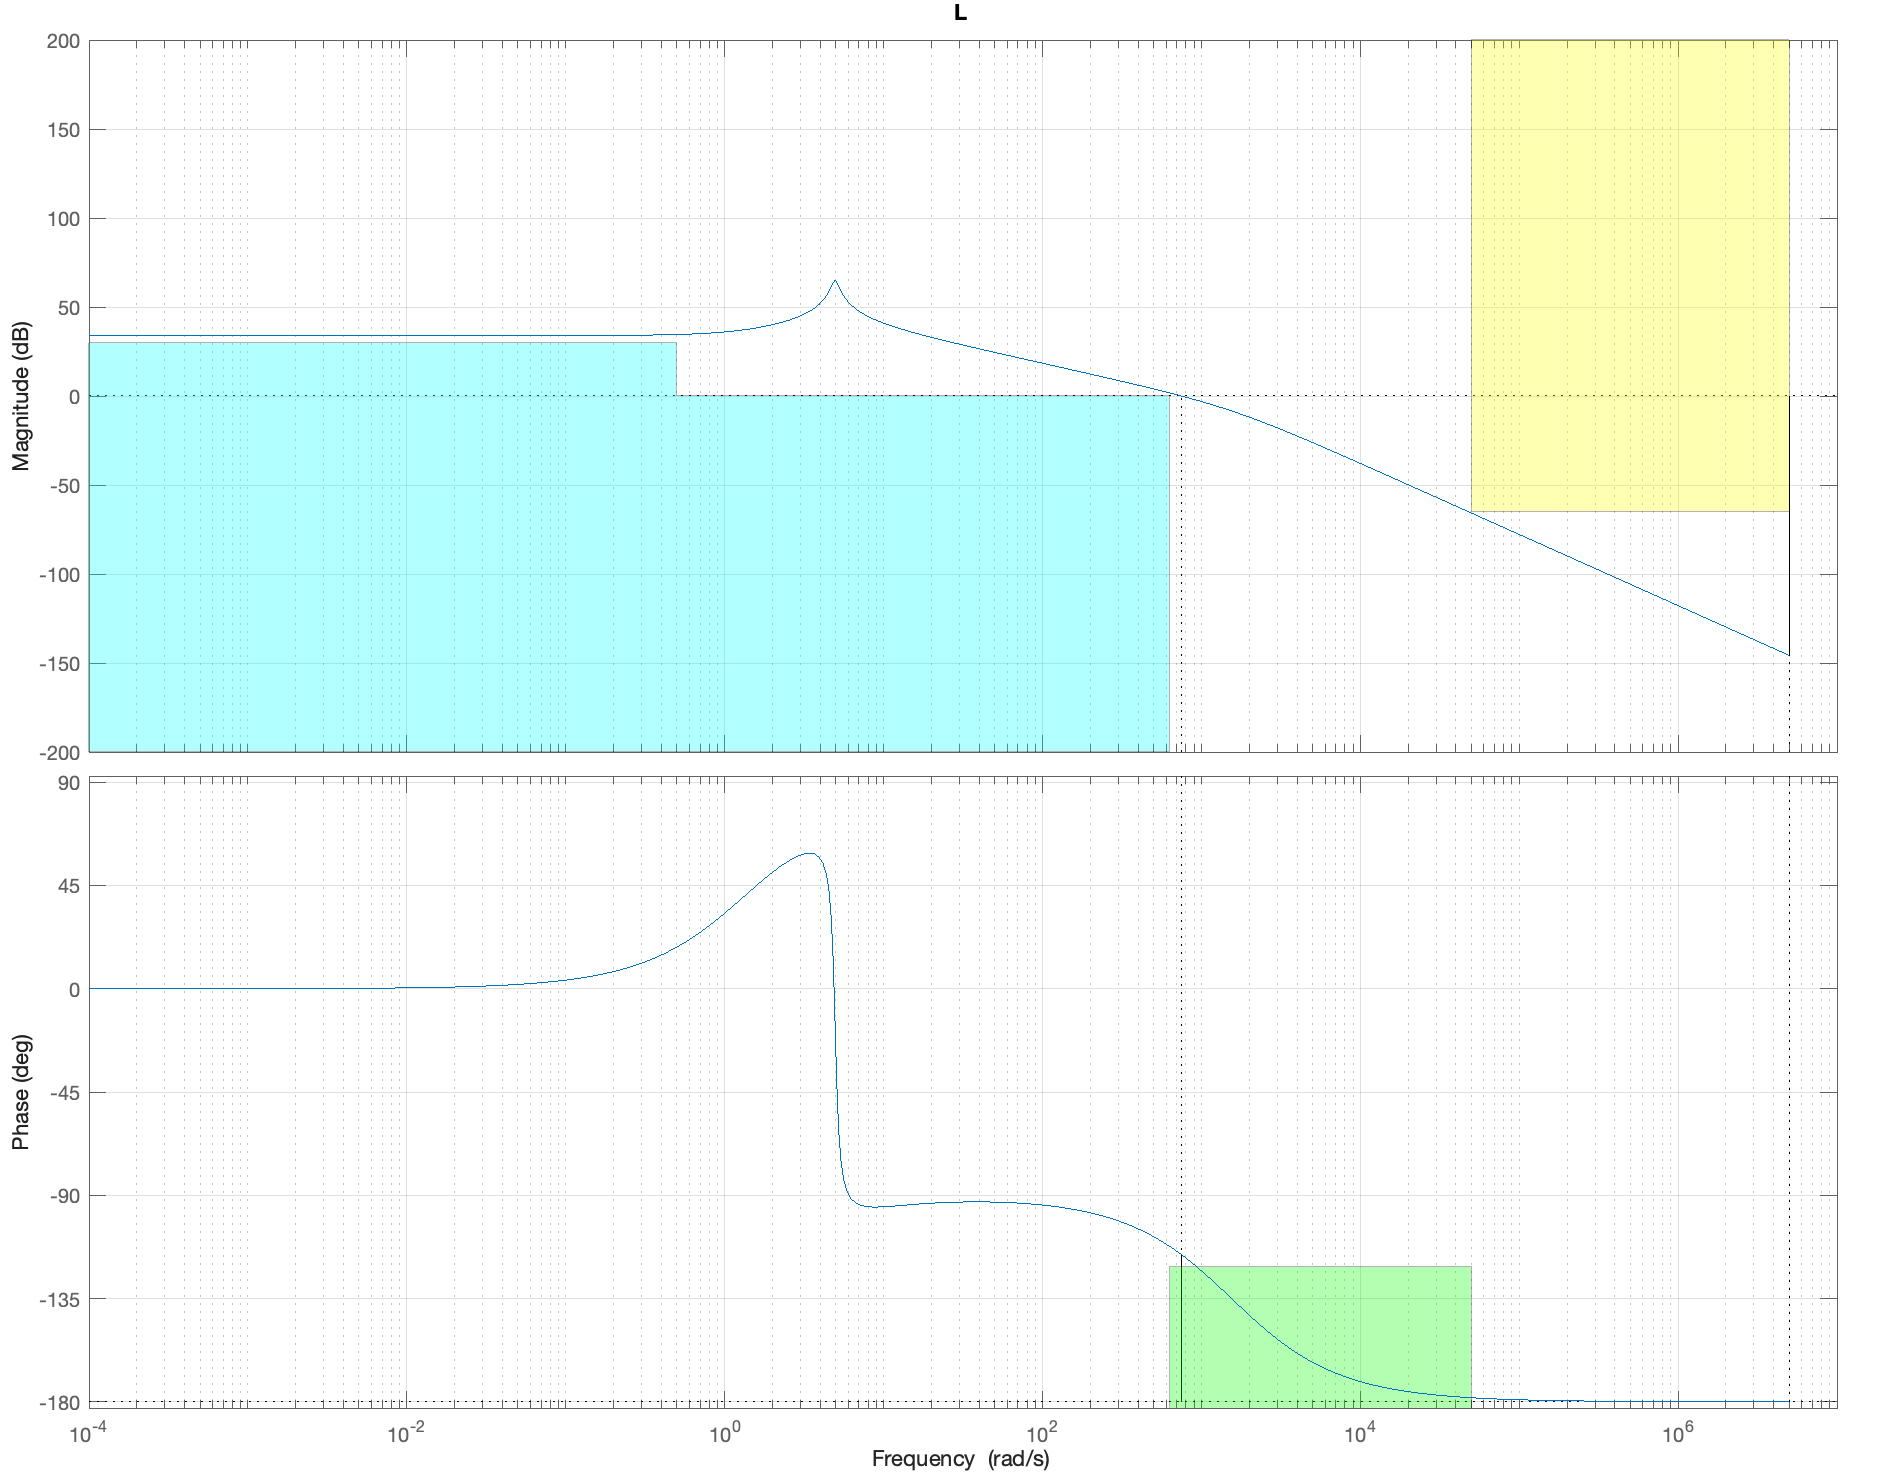
\includegraphics[width=0.75\linewidth]{./images/funzione_anello.png}
	\caption{Funzione d'anello L(s).}
	\label{fig:funzione_anello}
\end{figure}

\section{Test sul sistema linearizzato}

In questa sezione, testiamo l'efficacia del controllore progettato sul sistema linearizzato con $w(t) = 1(t)$, $d(t)=\sum_{k = 1}^{4} \sin(0.1kt)$ e $n(t)=\sum_{k = 1}^{4} \sin(5\space\cdot\space 10^{4}kt) $.

In Figura \ref{fig:step_response}, si mostra la risposta del sistema linearizzato ad un gradino unitario. \`E possibile notare come essa rispetti le specifiche richieste riguardanti tempo di assestamento, sovraelongazione e massimo errore a regime.
 
\begin{figure}[h!]
	\centering
	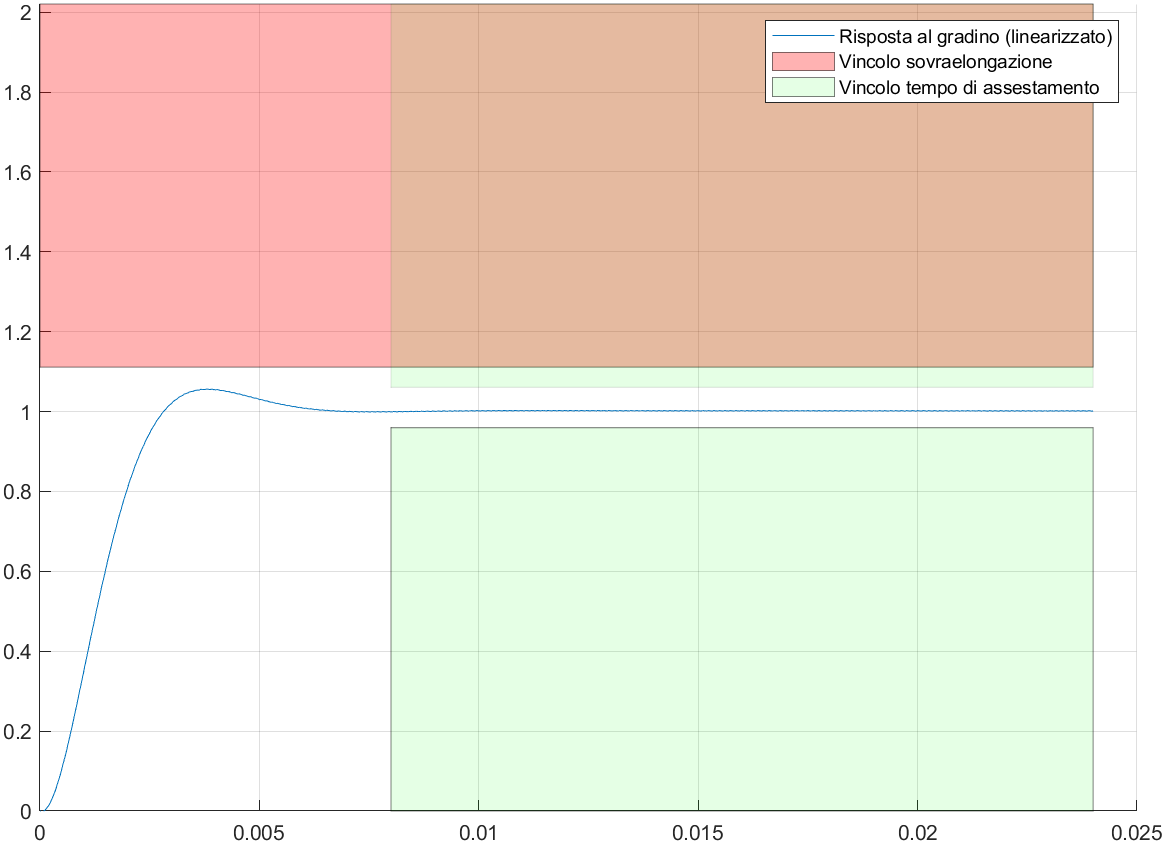
\includegraphics[width=0.9\linewidth]{./images/stepRespLin.png}
	\caption{Risposta del sistema linearizzato ad un gradino unitario.}
	\label{fig:step_response}
\end{figure}

Questo risultato \`e stato ottenuto progettando un regolatore statico $R_s(s)$ adeguato al fine di mantenere l'errore a regime inferiore ad un valore di $0.004$ (come spiegato nella Sezione~\ref{sec:static_regulator}) 
e un regolatore dinamico $R_d(s)$ che facesse s\`i che il sistema rispettasse un vincolo sul margine di fase $M_f$ tale per cui non si verificassero sovraelongazione e tempo di assestamento superiori alle specifiche richieste
(come spiegato nella Sezione~\ref{sec:dynamic_regulator}).

\section{Test sul sistema non lineare}

In questa sezione, testiamo l'efficacia del controllore progettato sul modello non lineare, tenendo anche conto della presenza di $d(t)$ ed $n(t)$.

\begin{figure}[h!]
	\centering
	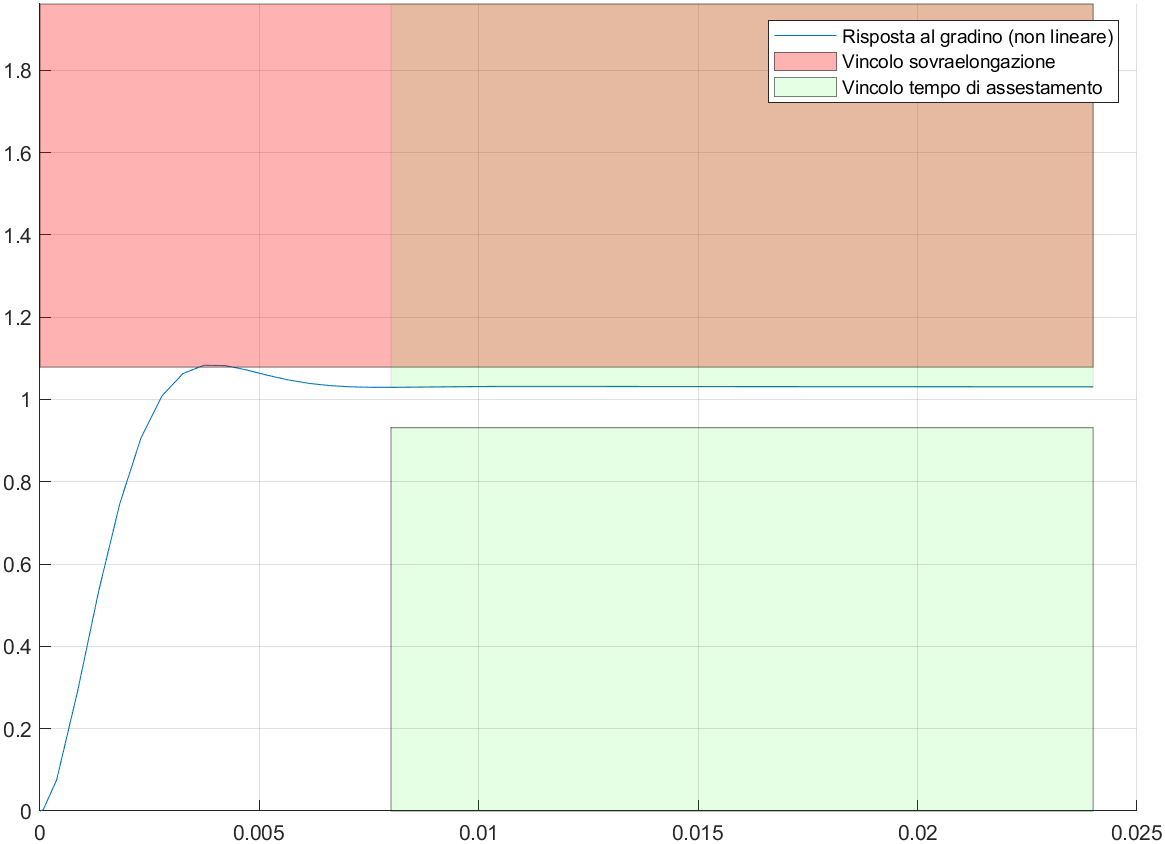
\includegraphics[width=0.9\linewidth]{./images/stepRespNonLinUni.png}
	\caption{Risposta del sistema non lineare ad un gradino unitario.}
	\label{fig:step_response_non_lin_uni}
\end{figure}

\section{Punti opzionali}

\subsection{Primo punto}

\dots 

\subsection{Secondo punto}

\dots

\subsection{Terzo punto}

\dots

\section{Conclusioni}

\dots

\end{document}
